% generated by make_figures.py
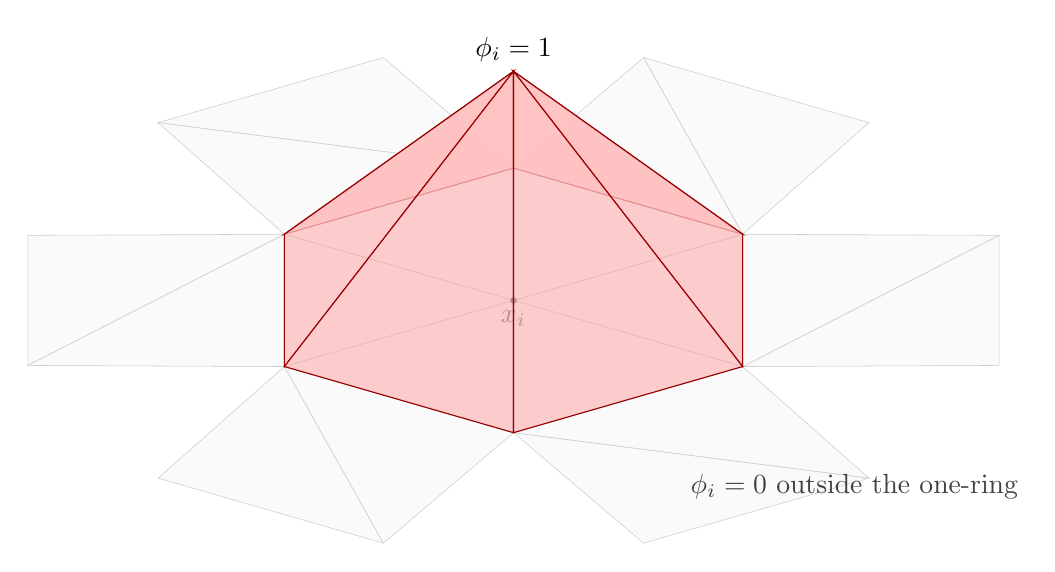
\begin{tikzpicture}[]
\filldraw[draw=gray!40, fill=gray!4, line width=0.2pt] (2.9098,-0.8400) -- (6.1665,-0.8262) -- (6.1665,0.8262) -- cycle;
\filldraw[draw=gray!40, fill=gray!4, line width=0.2pt] (2.9098,-0.8400) -- (6.1665,0.8262) -- (2.9098,0.8400) -- cycle;
\filldraw[draw=gray!40, fill=gray!4, line width=0.2pt] (2.9098,0.8400) -- (4.5142,2.2571) -- (1.6523,3.0832) -- cycle;
\filldraw[draw=gray!40, fill=gray!4, line width=0.2pt] (2.9098,0.8400) -- (1.6523,3.0832) -- (0.0000,1.6800) -- cycle;
\filldraw[draw=gray!40, fill=gray!4, line width=0.2pt] (0.0000,1.6800) -- (-1.6523,3.0832) -- (-4.5142,2.2571) -- cycle;
\filldraw[draw=gray!40, fill=gray!4, line width=0.2pt] (0.0000,1.6800) -- (-4.5142,2.2571) -- (-2.9098,0.8400) -- cycle;
\filldraw[draw=gray!40, fill=gray!4, line width=0.2pt] (-2.9098,0.8400) -- (-6.1665,0.8262) -- (-6.1665,-0.8262) -- cycle;
\filldraw[draw=gray!40, fill=gray!4, line width=0.2pt] (-2.9098,0.8400) -- (-6.1665,-0.8262) -- (-2.9098,-0.8400) -- cycle;
\filldraw[draw=gray!40, fill=gray!4, line width=0.2pt] (-2.9098,-0.8400) -- (-4.5142,-2.2571) -- (-1.6523,-3.0832) -- cycle;
\filldraw[draw=gray!40, fill=gray!4, line width=0.2pt] (-2.9098,-0.8400) -- (-1.6523,-3.0832) -- (0.0000,-1.6800) -- cycle;
\filldraw[draw=gray!40, fill=gray!4, line width=0.2pt] (0.0000,-1.6800) -- (1.6523,-3.0832) -- (4.5142,-2.2571) -- cycle;
\filldraw[draw=gray!40, fill=gray!4, line width=0.2pt] (0.0000,-1.6800) -- (4.5142,-2.2571) -- (2.9098,-0.8400) -- cycle;
\filldraw[draw=gray!60, fill=gray!8, line width=0.3pt] (0.0000,0.0000) -- (2.9098,-0.8400) -- (2.9098,0.8400) -- cycle;
\filldraw[draw=gray!60, fill=gray!8, line width=0.3pt] (0.0000,0.0000) -- (2.9098,0.8400) -- (0.0000,1.6800) -- cycle;
\filldraw[draw=gray!60, fill=gray!8, line width=0.3pt] (0.0000,0.0000) -- (0.0000,1.6800) -- (-2.9098,0.8400) -- cycle;
\filldraw[draw=gray!60, fill=gray!8, line width=0.3pt] (0.0000,0.0000) -- (-2.9098,0.8400) -- (-2.9098,-0.8400) -- cycle;
\filldraw[draw=gray!60, fill=gray!8, line width=0.3pt] (0.0000,0.0000) -- (-2.9098,-0.8400) -- (0.0000,-1.6800) -- cycle;
\filldraw[draw=gray!60, fill=gray!8, line width=0.3pt] (0.0000,0.0000) -- (0.0000,-1.6800) -- (2.9098,-0.8400) -- cycle;
\fill[fill=black] (0.0000,0.0000) circle (1.2pt) node[below] {$x_i$};
\filldraw[draw=red!60!black, fill=red!25, fill opacity=0.75, line width=0.4pt] (0.0000,2.9098) -- (0.0000,1.6800) -- (-2.9098,0.8400) -- cycle;
\filldraw[draw=red!60!black, fill=red!25, fill opacity=0.75, line width=0.4pt] (0.0000,2.9098) -- (2.9098,0.8400) -- (0.0000,1.6800) -- cycle;
\filldraw[draw=red!60!black, fill=red!25, fill opacity=0.75, line width=0.4pt] (0.0000,2.9098) -- (-2.9098,0.8400) -- (-2.9098,-0.8400) -- cycle;
\filldraw[draw=red!60!black, fill=red!25, fill opacity=0.75, line width=0.4pt] (0.0000,2.9098) -- (2.9098,-0.8400) -- (2.9098,0.8400) -- cycle;
\filldraw[draw=red!60!black, fill=red!25, fill opacity=0.75, line width=0.4pt] (0.0000,2.9098) -- (-2.9098,-0.8400) -- (0.0000,-1.6800) -- cycle;
\filldraw[draw=red!60!black, fill=red!25, fill opacity=0.75, line width=0.4pt] (0.0000,2.9098) -- (0.0000,-1.6800) -- (2.9098,-0.8400) -- cycle;
\node[above] at (0.0000,2.9098) {$\phi_i = 1$};
\node[right, gray!50!black] at (2.1253,-2.3594) {$\phi_i = 0$ outside the one-ring};
\end{tikzpicture}
